\documentclass[10pt,journal]{IEEEtran}

\usepackage{graphicx}
\usepackage{amsmath}
\usepackage{booktabs}
\usepackage{hyperref}
\usepackage{xcolor}
\usepackage{listings}
\usepackage{caption}

\hypersetup{colorlinks=true, linkcolor=blue, urlcolor=blue, citecolor=blue}

\lstset{
  basicstyle=\ttfamily\footnotesize,
  breaklines=true,
  columns=fullflexible,
  frame=single,
  backgroundcolor=\color{gray!8},
  keywordstyle=\color{blue!70!black},
  commentstyle=\color{gray!60!black}
}

\graphicspath{{figures/}}

\begin{document}

\title{Project Documentation: A Rosenthal Moving Heat Source Melt-Pool Calculator\\
\large for Laser Powder Bed Fusion}

\author{Adeleke Olorunnisola Oyeyemi\\
\textit{Department of Mechanical Engineering, Federal University of Technology, Akure, Nigeria}\\
Source code: \url{https://github.com/Olorunnisola01/rosenthal-meltpool}\\
Interactive demo: \url{https://rosenthal-meltpool.streamlit.app}}

\markboth{Project 1 Documentation}{}

\maketitle

\begin{abstract}
This document describes Project 1 of a six-month research-preparation programme in metal additive manufacturing (AM) process modelling: a software tool that predicts single-track melt-pool geometry in laser powder bed fusion (L-PBF) from the classical Rosenthal moving point-heat-source solution. The tool is delivered as a plain, dependency-light Python package (for reuse in later projects and citation in written work) and as a public, interactive web calculator built with Streamlit and embedded on the author's academic portfolio site. This document explains the underlying physics, the software architecture, the four preset alloy systems (Ti-6Al-4V, 316L stainless steel, AlSi10Mg, and Inconel 718), and walks through three worked examples with figures generated directly by the tool. It closes with a frank discussion of the model's limitations, several of which were only discovered through the process of building and testing this tool rather than assumed in advance.
\end{abstract}

\section{Introduction and Motivation}

Predicting the dimensions of the melt pool produced by a single laser scan is the cheapest and fastest screening step available before committing to full process-parameter optimization in L-PBF. Melt-pool width governs safe hatch spacing between adjacent scan tracks; melt-pool depth governs whether successive powder layers remelt into one another well enough to avoid lack-of-fusion porosity. Both quantities can, in principle, be estimated from an analytical solution to the heat conduction equation for a point source moving at constant velocity across (or through) a solid --- the moving heat source solution first published by Rosenthal in 1946 \cite{rosenthal1946}.

This project implements that analytical solution as a small, well-documented software tool, for two reasons specific to the author's six-month AM research-preparation plan. First, it is the technical core of Project 2 (parameter sweeps and literature validation, documented separately) and of Paper 2 (an analytical melt-pool modelling manuscript). Second, it establishes a working pattern --- a plain Python module paired with a public interactive demo --- that later, more complex projects in the plan (metaheuristic optimizers, CNN defect classifiers, CFD simulations) will reuse.

\section{Theoretical Background}

\subsection{The Rosenthal Moving Point-Source Solution}

Consider a point heat source of absorbed power $Q$ moving at constant velocity $v$ along the $x$-axis across the surface of a semi-infinite solid. In a reference frame that moves with the source, the temperature field reaches a quasi-steady state given by

\begin{equation}
T(x,y,z) - T_0 = \frac{Q}{2\pi k R}\exp\!\left(-\frac{v(R+x)}{2\alpha}\right)
\label{eq:rosenthal}
\end{equation}

where $R = \sqrt{x^2+y^2+z^2}$ is the radial distance from the (instantaneous) source position, $x$ is the coordinate behind the source ($x<0$ is the trailing wake, $x>0$ is ahead of it), $k$ is thermal conductivity, $T_0$ is the ambient or preheat temperature, and $\alpha = k/(\rho c_p)$ is thermal diffusivity, with $\rho$ density and $c_p$ specific heat capacity. The absorbed power is $Q = \eta P$, where $P$ is nominal laser power and $\eta$ is absorptivity --- the fraction of incident power actually absorbed into the melt pool.

Equation~\ref{eq:rosenthal} has a closed form only because $k$, $\rho$, and $c_p$ are treated as constants. This is the standard simplifying assumption that makes the model fast enough for process-window screening, at the cost of ignoring their real temperature dependence.

\subsection{Melt-Pool Boundary and Dimensions}

The melt-pool boundary is the isotherm $T = T_{\text{melt}}$ (taken as the alloy's liquidus temperature). Because Eq.~\ref{eq:rosenthal} is transcendental in $R$, the pool's width, depth, and length are found by numerical root-finding (Brent's method) rather than in closed form:

\begin{itemize}
\item \textbf{Half-width}: solve $T(0, y, 0) = T_{\text{melt}}$ for $y$; width $= 2y$.
\item \textbf{Depth}: solve $T(0, 0, z) = T_{\text{melt}}$ for $z$.
\item \textbf{Length}: solve $T(x, 0, 0) = T_{\text{melt}}$ separately for $x>0$ (leading edge) and $x<0$ (trailing edge); length is their sum.
\end{itemize}

\section{Software Architecture}

The project is split deliberately into a dependency-light core library and a separate interactive layer, so the physics can be reused (and cited) independently of any GUI framework.

\subsection{Core Python Package (\texttt{rosenthal/})}

\begin{itemize}
\item \texttt{materials.py} --- a frozen dataclass \texttt{Material} holding constant thermophysical properties ($k$, $\rho$, $c_p$, $T_{\text{melt}}$) plus a literature source string, and a small registry of four preset alloys (Section~\ref{sec:materials}).
\item \texttt{model.py} --- the temperature field (Eq.~\ref{eq:rosenthal}) and the root-finding routine that extracts width, depth, and length from it.
\item \texttt{sweep.py} --- evaluates melt-pool dimensions over a power$\times$velocity grid, for building process maps (used in Project 2).
\item \texttt{validation.py} --- compares model output against published single-track measurements and includes an absorptivity-calibration search (used in Project 2).
\end{itemize}

The only third-party dependency of the core package is \texttt{scipy} (for root-finding). It requires no GUI toolkit, no plotting library, and no internet access, so it can be imported and unit-tested in any Python environment. A 19-test \texttt{pytest} suite covers the physics, the material presets, and known structural properties of the model (Section~\ref{sec:limitations}).

\subsection{Interactive Web Calculator}

A separate Streamlit application (\texttt{streamlit\_app/app.py}) imports the core package directly --- it does not reimplement any physics --- and adds:

\begin{itemize}
\item Sliders for laser power, scan velocity, absorptivity, and preheat temperature, plus a material dropdown;
\item A plan-view (surface, $z=0$) and a cross-section ($x=0$) temperature-field plot, both rendered at a fixed physical size with the zoom level auto-fit to each result;
\item Plain-language interpretation of the numeric results in terms of hatch spacing and interlayer bonding;
\item Explicit statements of model limitations, shown alongside the results rather than in a separate document.
\end{itemize}

The app is deployed on Streamlit Community Cloud and embedded directly on a project page of the author's academic portfolio site via an iframe, so the calculator is usable in-browser without installing anything.

\section{Materials Database}
\label{sec:materials}

Four alloys were selected to match the four dominant material systems in current L-PBF research and practice, and to match the scope of the author's accompanying literature review paper. Table~\ref{tab:materials} lists the constant (temperature-averaged) property values used, sourced from Mills' widely cited compilation of thermophysical properties for commercial alloys \cite{mills2002}.

\begin{table}[!t]
\centering
\caption{Preset material properties (temperature-averaged)}
\label{tab:materials}
\begin{tabular}{@{}lrrrr@{}}
\toprule
Alloy & $k$ (W/m$\cdot$K) & $\rho$ (kg/m$^3$) & $c_p$ (J/kg$\cdot$K) & $T_{\text{melt}}$ (K) \\
\midrule
Ti-6Al-4V & 6.7 & 4430 & 526 & 1928 \\
316L & 21.5 & 8000 & 500 & 1710 \\
AlSi10Mg & 113.0 & 2670 & 900 & 870 \\
IN718 & 11.4 & 8190 & 435 & 1609 \\
\bottomrule
\end{tabular}
\end{table}

Three alloys (Ti-6Al-4V, 316L, AlSi10Mg) were chosen as the most common L-PBF alloys with the best-validated single-track literature data; Inconel 718 was added as a fourth because nickel superalloys are the other major L-PBF material family, relevant to aerospace applications.

\section{Worked Examples}

Three examples below were generated directly by the calculator (both the Python package and the deployed web app produce identical numbers, since the web app imports the package rather than reimplementing it). Each figure is a plan-view temperature field at the build surface ($z=0$); the cyan contour marks the predicted melt-pool boundary ($T=T_{\text{melt}}$) and the star marks the instantaneous laser position.

\subsection{Example 1: Ti-6Al-4V at Default Parameters}

Power $=200$~W, velocity $=800$~mm/s, absorptivity $=0.4$, preheat $=300$~K. The model predicts width $=54.1$~\textmu m, depth $=27.1$~\textmu m, length $=1182.8$~\textmu m.

\begin{figure}[!t]
\centering
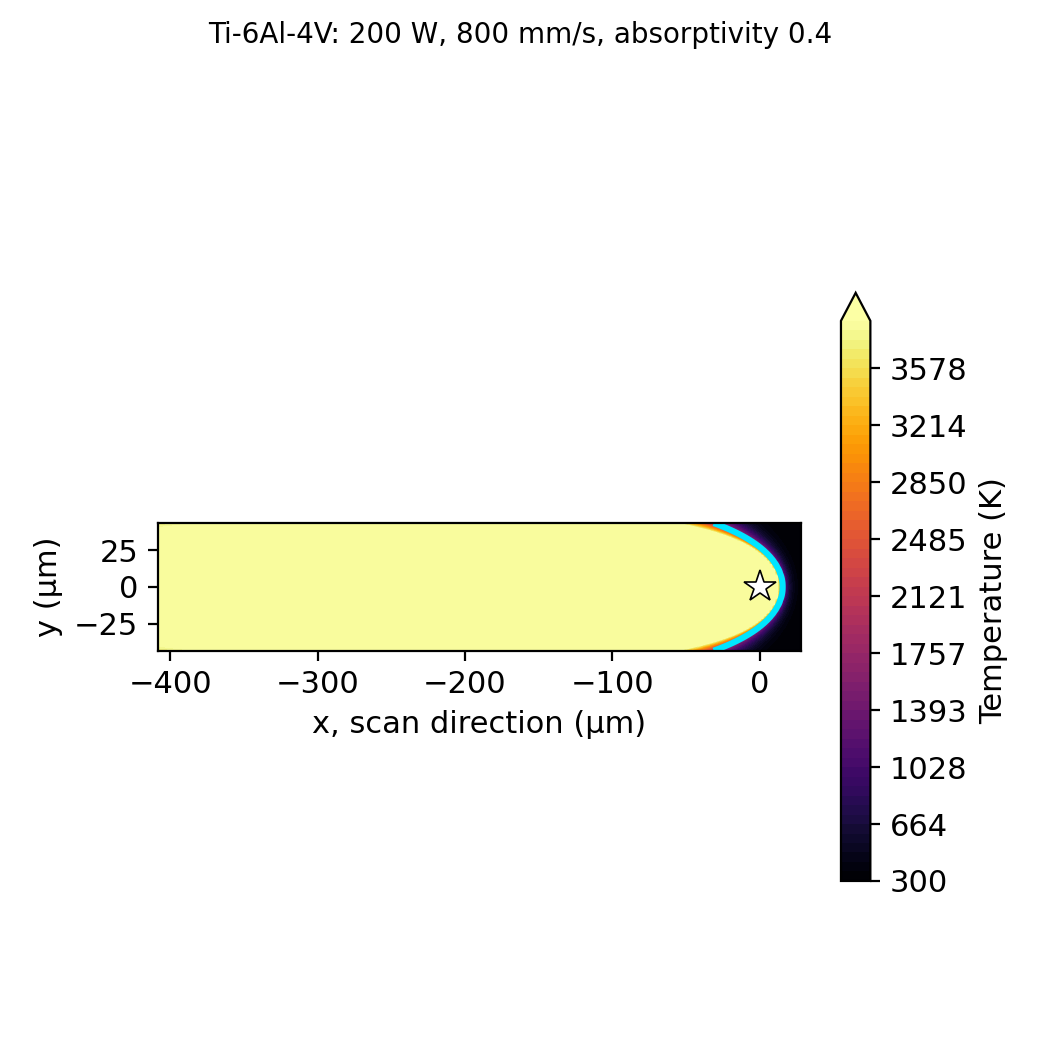
\includegraphics[width=\columnwidth]{example1_ti64_default.png}
\caption{Ti-6Al-4V plan view at default parameters. Note the pronounced trailing tail relative to pool width --- this is not a rendering artifact but a known structural property of the point-source model, discussed in Section~\ref{sec:limitations}.}
\label{fig:ex1}
\end{figure}

Fig.~\ref{fig:ex1} illustrates, more clearly than any of the other examples, a limitation discovered while building this tool: the predicted trailing length (1182.8~\textmu m) is over twenty times the predicted width. This is a deliberate choice of example, not a favourable one, because it is the clearest available illustration of the length-artifact limitation described in Section~\ref{sec:limitations}.

\subsection{Example 2: 316L at a Literature-Matched Parameter Set}

Power $=260$~W, velocity $=520$~mm/s, absorptivity $=0.5$, preheat $=300$~K --- chosen to match case N01 of a published single-track dataset for 316L \cite{zhang2024}, so the prediction can be compared directly against a real measurement. The model predicts width $=105.8$~\textmu m and depth $=52.9$~\textmu m; the published measurement for this exact parameter set is width $=114.0$~\textmu m and depth $=180.0$~\textmu m.

\begin{figure}[!t]
\centering
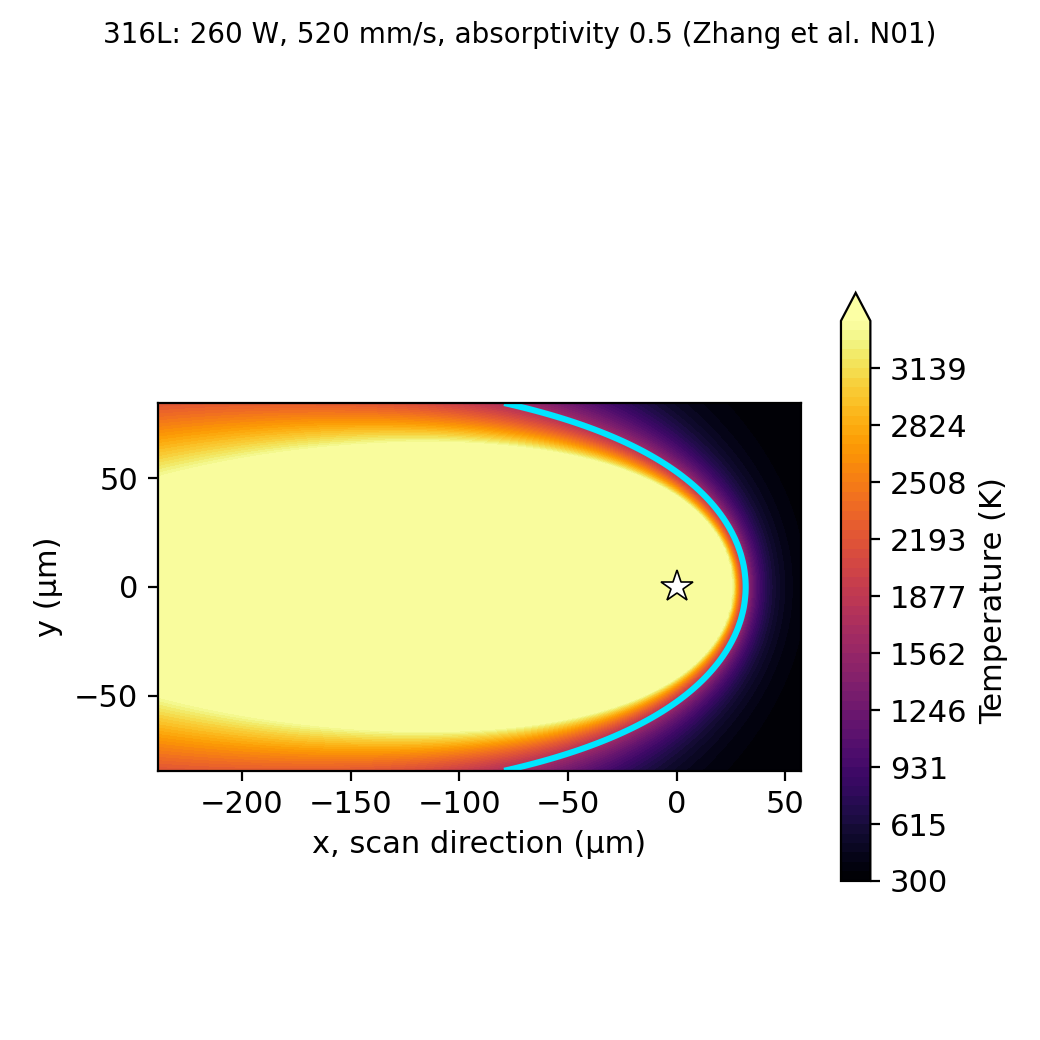
\includegraphics[width=\columnwidth]{example2_316L_validation_N01.png}
\caption{316L plan view at parameters matching Zhang et al.\ (2024) case N01. Predicted width is close to the measured value ($-7.2\%$); predicted depth is substantially below the measured value ($-70.6\%$), because this case is keyhole-influenced (measured depth exceeds measured width) and this model is conduction-mode only.}
\label{fig:ex2}
\end{figure}

Fig.~\ref{fig:ex2} is included specifically because it is a case where the model's prediction is known, from independent published data, to be inaccurate in depth --- this is more informative than showing only cases where the model happens to agree with experiment. A full validation study spanning four published cases is documented separately as Project 2.

\subsection{Example 3: AlSi10Mg at Default Parameters}

Power $=200$~W, velocity $=800$~mm/s, absorptivity $=0.4$, preheat $=300$~K. The model predicts width $=182.2$~\textmu m, depth $=91.1$~\textmu m, length $=262.9$~\textmu m.

\begin{figure}[!t]
\centering
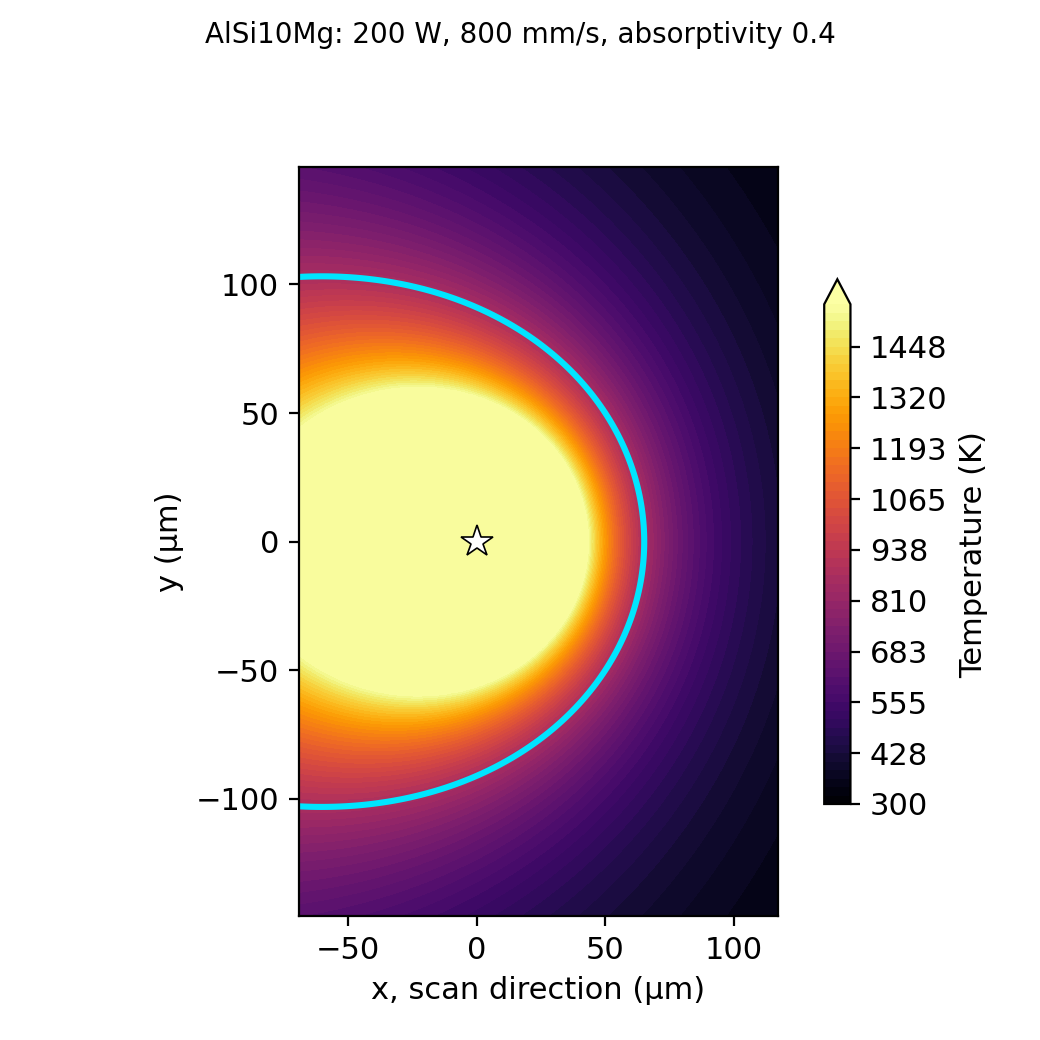
\includegraphics[width=\columnwidth]{example3_alsi10mg_default.png}
\caption{AlSi10Mg plan view at default parameters. AlSi10Mg's high thermal conductivity (113~W/m$\cdot$K, roughly 17$\times$ that of Ti-6Al-4V) spreads heat laterally far more efficiently, producing a visibly wider, shallower, and less elongated pool at identical process parameters than either other example.}
\label{fig:ex3}
\end{figure}

Fig.~\ref{fig:ex3} was chosen deliberately as a contrast to Fig.~\ref{fig:ex1}: identical process parameters (200~W, 800~mm/s, absorptivity 0.4) produce a pool over three times wider and with a far more proportionate, less elongated shape, purely because of the alloy's different thermal conductivity. This pairing is the clearest single illustration in this document of why material choice, not only process parameters, drives melt-pool geometry.

\section{Model Limitations}
\label{sec:limitations}

Several limitations below were established quantitatively through building and testing this tool, not assumed from the literature in advance.

\subsection{Conduction-Mode Only}

The model does not capture keyhole-mode vaporization, recoil pressure, or Marangoni convection. It also assumes constant (not temperature-dependent) thermophysical properties. Predictions should be treated as first-pass estimates for comparing process parameters against each other, not as a substitute for a validated thermal-fluid simulation.

\subsection{Depth-to-Width Ratio is Always Exactly 0.5}

The most significant limitation found during development is a provable mathematical identity, not an approximation: at the source's cross-section ($x=0$), the equation solved for half-width (along $y$) and the equation solved for depth (along $z$) are literally identical, because $R=\sqrt{y^2+z^2}$ at $x=0$ treats the two directions interchangeably. Consequently, \textbf{depth $=$ half-width, and depth/width $\equiv 0.5$, for every material and every parameter combination this model can be given} --- confirmed numerically across all four preset alloys and wide parameter ranges (see the project's test suite). The predicted cross-section is therefore always a perfect semicircle by construction.

Real melt pools are not semicircular: conduction-mode pools tend to run shallower than 0.5, while keyhole-mode pools run deeper, sometimes exceeding an aspect ratio of 1 (deeper than wide). The published validation data used in Example 2 spans measured aspect ratios from 0.49 to 1.58 across four cases, none of which this model can reproduce regardless of parameter or absorptivity choice. Reproducing a non-0.5 aspect ratio requires a structurally different heat-source model, such as Goldak's double-ellipsoidal source \cite{goldak1984}, not a parameter adjustment to this one.

\subsection{Trailing-Centerline Length Artifact}

Exactly on the trailing centerline behind the source ($y=0$, $z=0$, $x<0$), $R=-x$, so $R+x=0$ identically along that entire line, and the exponential decay term in Eq.~\ref{eq:rosenthal} degenerates to 1. Temperature there falls off only as $1/R$ rather than exponentially, which makes predicted pool length --- and only length, not width or depth --- substantially larger than real single-track measurements. Example 1 (Fig.~\ref{fig:ex1}) was chosen specifically to make this visible. Width and depth remain the reliable outputs of this model; length should be used only for relative comparison between parameter sets.

\subsection{Absorptivity Is Necessary but Not Sufficient}

Absorptivity is the one input that cannot be read directly from a material datasheet, and is the natural first parameter to adjust when a prediction disagrees with experiment. However, a calibration search performed as part of Project 2 shows this is not always sufficient: for three of the four published validation cases, no absorptivity value up to 500\% (a physically implausible value, tested deliberately to establish an upper bound) closes the gap between predicted and measured dimensions. The root cause is that predicted pool sizes in those cases (35--115~\textmu m) are comparable to the real laser spot diameter (100~\textmu m) reported in the source study --- the point-source assumption requires pool size to be much larger than source size, a condition these cases do not satisfy.

\section{Conclusion}

This project delivers a small, well-tested, and honestly documented implementation of a classical analytical melt-pool model, in a form usable both as a citable Python library and as a public interactive demonstration. Its value lies not only in the calculator itself but in the quantitative limitations established while building it --- in particular, the exact depth/width$=0.5$ identity and the bounded failure of absorptivity calibration --- both of which directly motivate the process-map sweep and literature validation carried out in Project 2, and the discussion of appropriate heat-source models for future, more physically complete work.

\begin{thebibliography}{9}

\bibitem{rosenthal1946}
D. Rosenthal, ``The theory of moving sources of heat and its application to metal treatments,'' \textit{Trans. ASME}, vol. 68, pp. 849--866, 1946.

\bibitem{mills2002}
K. C. Mills, \textit{Recommended Values of Thermophysical Properties for Selected Commercial Alloys}. Cambridge, U.K.: Woodhead Publishing, 2002.

\bibitem{zhang2024}
S. Zhang \textit{et al.}, ``Understanding melt pool behavior of 316L stainless steel in laser powder bed fusion additive manufacturing,'' \textit{Micromachines}, vol. 15, no. 2, p. 170, 2024, doi: 10.3390/mi15020170.

\bibitem{goldak1984}
J. Goldak, A. Chakravarti, and M. Bibby, ``A new finite element model for welding heat sources,'' \textit{Metallurgical Transactions B}, vol. 15, no. 2, pp. 299--305, 1984.

\end{thebibliography}

\end{document}
